\documentclass[twocolumn]{article}
% Fonts and typesetting settings
\usepackage[sc]{mathpazo}
\usepackage[T1]{fontenc}
\linespread{1.05} % Palatino needs more space between lines
\usepackage{microtype}
% Page layout
\usepackage[hmarginratio=1:1,top=32mm,columnsep=20pt]{geometry}
\usepackage[font=it]{caption}
\usepackage{paralist}
% Lettrines
\usepackage{lettrine}
% Abstract
\usepackage{abstract}
	\renewcommand{\abstractnamefont}{\normalfont\bfseries}
	\renewcommand{\abstracttextfont}{\normalfont\small\itshape}
% Titling (section/subsection)
\usepackage{titlesec}
\renewcommand\thesection{\Roman{section}}
\titleformat{\section}[block]{\large\scshape\centering}{\thesection.}{1em}{}
% Math Packages
\usepackage{amsmath}
\usepackage{amsfonts}
\usepackage{amssymb}
\newcommand{\xor}{\oplus}
% Header/footer
\usepackage{fancyhdr}
	\pagestyle{fancy}
	\fancyhead{}
	\fancyfoot{}
	\fancyhead[C]{Introduction to Cryptographic Algorithms $\bullet$ Assignment: Short Paper}
%including sourcecode in text
\usepackage{verbatim}

% ------
% Clickable URLs (optional)
\usepackage{hyperref}
% ------
% Maketitle metadata
\title{\vspace{-15mm}%
	\fontsize{24pt}{10pt}\selectfont
	\textbf{Summary of:\\Plaintext Recovery Attacks against SSH}
	}	
\author{%
	\large
	\textsc{Raoul Estourgie} \\[2mm]
	\normalsize	Radboud University Nijmegen \\
	\normalsize	s3022420
	\vspace{-5mm}
	\and 
	\large
	\textsc{Ben Br\"ucker} \\[2mm]
	\normalsize	Radboud University Nijmegen \\
	\normalsize	s0413291
	\vspace{-5mm}
	}
\date{}
\bibliographystyle{ieeetran}
\usepackage[pdftex]{graphicx}
%%%%%%%%%%%%%%%%%%%%%%%%


\begin{document}

\twocolumn[\begin{@twocolumnfalse}
  \maketitle
  \begin{abstract}
  \noindent We are summarizing the article "Plaintext Recovery Attacks against SSH" by Martin R. Albrecht, Kenneth G. Paterson and Gaven J. Watson~\cite{Albrecht2009}. In this article they discuss a weakness in the OpenSSH protocol that allows an adversary to extract plaintext bits. We are going to summarize the key parts of that paper in order to present their findings to our class.
\end{abstract}
\end{@twocolumnfalse}]

\thispagestyle{fancy}

\lettrine[nindent=0em,lines=3]{S} ecure Shell (SSH) connects computers over securely over insecure network connections~\cite{Ylonen2006}. This protocol was released in 1995 and was designed to replace rlogin, rsh, Telnet and similar insecure protocols. 
\indent The SSH protocol covers Authentication, Confidentiality and Integrity~\cite{Barret2001}.
\indent The "Plaintext Recovery Attacks against SSH" paper~\cite{Albrecht2009} focuses on the OpenSSH implementation of the SSH Binary Packet Protocol (BPP).

\section{The SSH-BPP protocol}
\indent The Binary Packet Protocol (BPP) of SSH encrypts the plaintext and then protects the integrity by appending a MAC value~\cite{Ylonen2006}.

\indent Before encryption, the message is encoded by prefixing a 4 byte packet length field and a 1 byte padding length field. At least 4 bytes of randomized padding must be added as a suffix with a maximum of 255 bytes~\cite{Albrecht2009}. The message is then encrypted with a cypher of choice, for example aes128-cbc. After that, a MAC value is added. This MAC is computed from the cyphertext and a 32-bit packet sequence number. (See figure ~\ref{fig:BPPProtocol})

\indent The packets then form a data stream since the encryption is in CBC mode. Every packet $i-1$ on a connection will be the initialization vector IV for packet $i$ on the same connection~\cite{Albrecht2009}.

\indent For decryption it is essential that the receiver decrypts the first ciphertext block to be able to read the length field. Without this he does not know when a complete packet has arrived and when to perform the MAC check. Most SSH implementations wait until enough data has arrived to complete the packet~\cite{Albrecht2009}.

\indent The SSH protocol~\cite{Ylonen2006} also specifies error handling for the BPP protocol. The connection should terminate whenever a transmission error occurs or MAC verification fails. After that the connection should be re-established. Implementations are free to send error messages to their peer when an error occurs.

\begin{figure*}
	  \centering
    	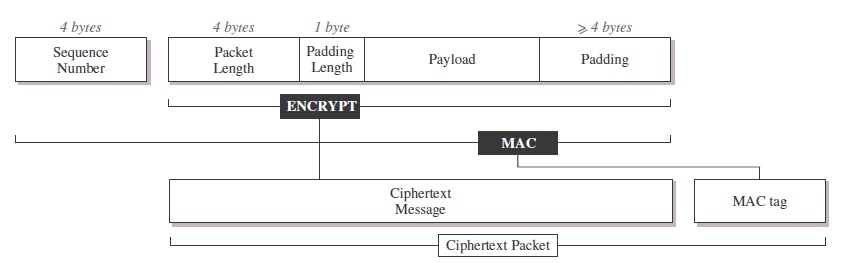
\includegraphics[scale=.6]{SSHBPP.png}
	\caption{SSH BPP packet format and cryptographic processing~\cite{Albrecht2009}}
	\label{fig:BPPProtocol}
\end{figure*}

\section{Open SSH implementation of the BPP protocol}

\indent Open SSH follows the guidelines for BPP fairly close~\cite{Albrecht2009}. But the details are important since they are a the focus of the attack.

\indent After receiving the first ciphertext block, Open SSH first performs a length check. If the length given in the length field is not greater then 5 and less then $2^{18}$ it sends a \textit{SSH2 MSG DISCONNECTED} error back to the sender.

\indent Then OpenSSH checks that the total number of bytes expected is indeed a multiple of the block size. If this check fails, the TCP connection will terminate without error message~\cite{Albrecht2009}.

\indent Lastly, OpenSSH performs a MAC check when all data for the package has arrived. If this check fails, a \textit{Corrupted MAC on input.} error message is returned to the sender.

\indent Albrecht et al.~\cite{Albrecht2009} note that further checks performed by OpenSSH are not of interest for their attack. Further it is important to note that Each of the checks has a different type of error behavior, that can be used to facilitate their attack.




\section{The Attack}
\subsection*{general overview}
SSH bpp makes use of a block cipher in CBC mode to provide confidentiality. Cipher Block Chaining (CBC) is an invention of IBM, it is a tool to make your current message you are decrypting/encrypting dependant on all the previous encrypted messages. To guarantee the integrity of the data a MAC algorithm is used to create a MAC-tag that is added to the rest of the packet. The protocol includes a 32-bit packet length field which appears in encrypted form in the first block of ciphertext in the SSH packet. This can be exploited to recover plaintext from an enciphered text. By sending a target ciphertext block as the first block of a new SSH packet, the attacker can induce the SSH server to treat the resulting plaintext as the first block of a new packet. All you then need to do is feed the server random blocks of ciphertext into the SSH connection. The attacker can now meassure how much data is required before the server thinks the whole packet has arrived. It will then check the MAC, and will produce a MAC failure (because we have been feeding random packets this is almost a probability of 1). The server will then produce an error and shutdown the connection. This error message reveals the 32-bit encrypted packet length field, because we know exactly how much data is sent to the server. The chaining property of the CBC mode helps us to acquire an extra 32-bits. An unfortunate feature from this attack is that the adversary needs to send $2^{27}$ ciphertext blocks on average before the MAC check is triggered. But the attack would succeed with a probability of 1 and can be done with any of the encrypted ssh packets.
\subsection{complications of the attack}
Open SSH checks if the packet length field is at most $2^{18}$ and then checks if it has a certain divisibility property. The connection is torn down if either check fails. The effect of the length checking will reduce the success of the attack to about $2^{-18}$. However the effect is that it reduces the maximum number the attacker has to inject to only $2^{14}$.
\subsection{notation}
Let us first define some notation. K is the key of our block cipher, which is fixed for the duration of a connection. $F_k$ and $F^{-1}_k$ are the encryption and decryption operations of the block cipher. L is the block size of the block cipher in bytes. The CBC mode in SSH BPP then operates as follows: given a sequence $p_1,p_2,...,p_n$ of plaintext blocks making up a packet, we have: 
$c_i = F_k(c_{i-1} \oplus p_i), i = 1,2,...,n$
where $c_0$, the Initializing Vector (IV), is taken as the last block of the previous ciphertext. Decription works as follows:
$p_i = c_{i-1} \oplus F^{-1}_k(c_i), i = 1,2,...,n$
\subsection{the attack}
The attacker collects a target ciphertext block $c_i^*$ from an established SSH connection. Let $c_{i-1}^*$ denote the preceding target block and $p_i^*$ denote the target plaintext of $c_i^*$.
$p_i^* = c_{i-1}^* \oplus F^{-1}_k(c_i^*)$
The attacker now injects $c_i^*$ as the first block of a new packet. Let $c_n$ denote the last ciphertext block of the preceding packet on the connection. This block is used as the IV for the new packet, so the will receive $p^{'}_1$ after decryption because:
$p^{'}_1 = c_n \oplus F^{-1}_k(c_i^*)$
By combining the equations, we get:
$p_i^* = c_{i-1}^* \oplus p^{'}_1 \oplus c_n$ (1)
After receiving $c_i^*$, there are two options. Either a termination of the TCP connection over which the connection is running, or the SSH connection enters a state in which it is waiting for more data. We then know that $p^{'}_1$ has passed the length check. This only occurs if the packet length field in $p^{'}_1$ lies between 5 and $2^{18}$, which only occurs if the first 14 bits of $p^{'}_1$ are zero, we can use this and the equation in (1) to calculate the first 14 bits of $p_i^*$. $p^{'}_1$ is a random 32-bit value, therefore the length check will pass with probability $2^{-14} - 5/2^{18} \approx 2^{-14}$. Which is a low chance but will give us the first 14 bits of $p^*_i$, and still is a way better chance then guessing.
\subsection{recovering 32 plaintext bits}
We now continue where we left at the second attack, the attacker retrieved 14 plaintext bits and now knows that the server is in a wait state. When L = 16 (e.g. with aes), this implies that the first 14 bits of the length field in $p^{'}_1$ will all be zero, and that the last 4 bits of this field encode the value 12. So we now have 18 bits we can use to calculate parts of $p^*_i$ using equation (1)(with 3des L = 8 and the last 3 bits of the length field should encode the value 4 which gives us 17 bits in total). When both test pass we no know that the server is waiting for more data until the following condition is no longer satisfied.
\begin{verbatim}
if (buffer_len(&input) < need + maclen)
	return SSH_MSG_NONE;
\end{verbatim}
Once the test fails, the MAC check will be triggered. The attacker continues his attack by injecting packets of size \emph{maclen}. The attacker will keep feeding the server packets until it receives a MAC error which is after at most $2^{18}/L$ packets. When this occurs we know the value of \emph{need}, the exact value of $p_1^{'}$.
\begin{verbatim}
need = 4 + packet_length - block_size
\end{verbatim}
Knowing this 32-bit value, the first 32 bits of $p^*_i$ can be recovered using equation (1).
The overall success probability is $2^{-18}$ with the recommended AES-CBC and $2^{-17}$ with the required 3des-CBC.
\subsection{Countermeassures}
One of the countermeasures openSSH took was to return the same message when the length check or the block check failed. This means that you can't apply the first attack to reveal the first 14 bits. However this doesn't prevent the 32-bit recovery attack. An extra improvement is to randomize the length field if the length check fails. The system then proceeds with the new length until the MAC check fails. This will causes a problem for our attacker since it now doesn't know if the length is accepted and the MAC tag just failed or the length isn't accepted and it just returns the MAC error.

\bibliography{Master}



\end{document}